\documentclass[12pt]{article}
\usepackage{graphicx,import}
\usepackage[svgnames]{xcolor} 
\usepackage{fancyhdr}
\usepackage{subfig}
\usepackage{hyperref}
\usepackage{enumitem}
\usepackage{cite}
\usepackage[many]{tcolorbox}
\usepackage{listings }
\usepackage[a4paper, total={6in, 8in} , bottom = 25mm , top = 25mm, headheight = 1.25cm , includehead,includefoot,heightrounded ]{geometry}
\usepackage{afterpage}
\usepackage{amssymb}
\usepackage{pdflscape}
\usepackage{gensymb}
\usepackage{textcomp}
\usepackage{tikz,pgfplots}
\usepackage{xecolor}
\usepackage{rotating}
\usepackage{pdfpages}
\usepackage[Kashida]{xepersian}
\usepackage[T1]{fontenc}
\usepackage{tikz}
\usepackage[utf8]{inputenc}
\usepackage{PTSerif} 
\usepackage{seqsplit}

\usepackage[edges]{forest}

\usepackage{listings}
\usepackage{xcolor}

\hypersetup{
	colorlinks   = true, %Colours links instead of ugly boxes
	urlcolor     = blue, %Colour for external hyperlinks
	linkcolor    = blue, %Colour of internal links
	citecolor   = red %Colour of citations
}
 
\definecolor{codegreen}{rgb}{0,0.6,0}
\definecolor{codegray}{rgb}{0.5,0.5,0.5}
\definecolor{codepurple}{rgb}{0.58,0,0.82}
\definecolor{backcolour}{rgb}{0.95,0.95,0.92}
 
\NewDocumentCommand{\codeword}{v}{
\texttt{\textcolor{blue}{#1}}
}
\lstset{language=java,keywordstyle={\bfseries \color{blue}}}

\lstdefinestyle{mystyle}{
    backgroundcolor=\color{backcolour},   
    commentstyle=\color{codegreen},
    keywordstyle=\color{magenta},
    numberstyle=\tiny\color{codegray},
    stringstyle=\color{codepurple},
    basicstyle=\ttfamily\normalsize,
    breakatwhitespace=false,         
    breaklines=true,                 
    captionpos=b,                    
    keepspaces=true,                 
    numbers=left,                    
    numbersep=5pt,                  
    showspaces=false,                
    showstringspaces=false,
    showtabs=false,                  
    tabsize=2
}

\lstset{style=mystyle}

\settextfont[Scale=1.2 ,BoldFont={Bahij Nazanin-Bold.ttf} , ItalicFont = {IRNazaninIranic.ttf}]{Bahij Nazanin-Regular.ttf}
\setlatintextfont[Scale = 1.0]{Garamond}
\DefaultMathsDigits 
\DeclareMathSizes{11}{19}{13}{9} 
%\DeclareMathSizes{12}{14.4}{8}{9}





\newenvironment{changemargin}[2]{%
\begin{list}{}{%
\setlength{\topsep}{0pt}%
\setlength{\leftmargin}{#1}%
\setlength{\rightmargin}{#2}%
\setlength{\listparindent}{\parindent}%
\setlength{\itemindent}{\parindent}%
\setlength{\parsep}{\parskip}%
}%
\item[]}{\end{list}}


\definecolor{foldercolor}{RGB}{124,166,198}

\tikzset{pics/folder/.style={code={%
    \node[inner sep=0pt, minimum size=#1](-foldericon){};
    \node[folder style, inner sep=0pt, minimum width=0.3*#1, minimum height=0.6*#1, above right, xshift=0.05*#1] at (-foldericon.west){};
    \node[folder style, inner sep=0pt, minimum size=#1] at (-foldericon.center){};}
    },
    pics/folder/.default={20pt},
    folder style/.style={draw=foldercolor!80!black,top color=foldercolor!40,bottom color=foldercolor}
}

\forestset{is file/.style={edge path'/.expanded={%
        ([xshift=\forestregister{folder indent}]!u.parent anchor) |- (.child anchor)},
        inner sep=1pt},
    this folder size/.style={edge path'/.expanded={%
        ([xshift=\forestregister{folder indent}]!u.parent anchor) |- (.child anchor) pic[solid]{folder=#1}}, inner xsep=0.6*#1},
    folder tree indent/.style={before computing xy={l=#1}},
    folder icons/.style={folder, this folder size=#1, folder tree indent=3*#1},
    folder icons/.default={12pt},
}

\begin{document}


%%% title pages
\begin{titlepage}
\begin{center}
        
\vspace*{0.7cm}


\includegraphics[width=0.4\textwidth]{sharif1.png}\\
\vspace{0.5cm}
\textbf{ \Huge{\emph ‌سیگنال‌ها و سیستم‌ها} }\\
\vspace{0.5cm}
\textbf{ \Large{ تمرین چهارم} }
\vspace{0.2cm}
       
 
      \large \textbf{دانشکده مهندسی کامپیوتر}\\\vspace{0.2cm}
    \large   دانشگاه صنعتی شریف\\\vspace{0.2cm}
       \large   ﻧﯿﻢ سال دوم 00-99 \\\vspace{0.2cm}
      \noindent\rule[1ex]{\linewidth}{1pt}
استاد:\\
    \textbf{{جناب آقای دکتر منظوری شلمانی}}


    \vspace{0.15cm}
نام و نام خانوادگی:\\

       
    \textbf{{امیرمهدی نامجو - 97107212}}
\end{center}
\end{titlepage}
%%% title pages


%%% header of pages
\newpage
\pagestyle{fancy}
\fancyhf{}
\fancyfoot{}
\cfoot{\thepage}
\chead{تمرین چهارم}
\rhead{
\includegraphics[width=0.1\textwidth]{sharif.png}}
\lhead{امیرمهدی نامجو}
%%% header of pages

\KashidaOff

\section{سوال اول}


\begin{enumerate}
	\item
	$$H_1(e^{j\omega}) = \frac{1+\frac{1}{2} e^{-j\omega}}{1+\frac{1}{4} e^{-j\omega}} = \frac{1 + \frac{1}{2} \cos (\omega) - j \frac{1}{2}\sin(\omega)}{1 + \frac{1}{4} \cos(\omega) - j \frac{1}{4} \sin (\omega)}$$
	$$|H_1(e^{jw})| =  \frac{(1 + \frac{1}{2} \cos (\omega))^2 +  (\frac{1}{2}\sin(\omega))^2}{(1 + \frac{1}{4} \cos(\omega))^2 + ( \frac{1}{4} \sin (\omega))^2}$$
	$$=\frac{\frac{5}{4}+ \cos (\omega)}{\frac{17}{16} + \frac{1}{2}\cos (\omega)}$$
	
	
	$$
H_{2}\left(e^{j \omega}\right) =\frac{\frac{1}{2}+e^{-j \omega}}{1+\frac{1}{4} e^{-j \omega}} \\
=\frac{\frac{1}{2}+\cos (\omega)-j \sin (\omega)}{1+\frac{1}{4} \cos (\omega)-j \frac{1}{4} \sin (\omega)}
	$$
	
	$$
	\left|H_{2}\left(e^{j \omega}\right)\right|=\frac{\left(\frac{1}{2}+\cos (\omega)\right)^{2}+\sin ^{2}(\omega)}{\left(1+\frac{1}{4} \cos (\omega)\right)^{2}+\left(\frac{1}{4} \sin (\omega)\right)^{2}}
	$$
	
	$$=\frac{\frac{5}{4}+ \cos (\omega)}{\frac{17}{16} + \frac{1}{2}\cos (\omega)}$$
		
	$$|H_1(e^{j\omega})| = |H_2(e^{j\omega})|$$	
		
		یعنی برابرند.
		
	\item
	
	$$\angle H_1 (e^{j \omega}) = -\tan^{-1} (\frac{\frac{1}{2} \sin (\omega)}{1 + \frac{1}{2} \cos (\omega)}) - (-\tan^{-1} (\frac{\frac{1}{4} \sin (\omega)}{1 + \frac{1}{4} \cos (\omega)}))$$
	$$= -\tan^{-1} (\frac{\frac{1}{2} \sin (\omega)}{1 + \frac{1}{2} \cos (\omega)}) + \tan^{-1} (\frac{\frac{1}{4} \sin (\omega)}{1 + \frac{1}{4} \cos (\omega)}))$$
	
	$$\angle H_2 (e^{j \omega}) = -\tan^{-1} (\frac{ \sin (\omega)}{\frac{1}{2} +  \cos (\omega)}) - (-\tan^{-1} (\frac{\frac{1}{4} \sin (\omega)}{1 + \frac{1}{4} \cos (\omega)}))$$
	$$= -\tan^{-1} (\frac{ \sin (\omega)}{\frac{1}{2} +  \cos (\omega)}) +\tan^{-1} (\frac{\frac{1}{4} \sin (\omega)}{1 + \frac{1}{4} \cos (\omega)}))$$
	
	تاخیر گروه به نوعی منفی نرخ تغییرات فاز نسبت به $\omega$ است.
	
	اگر از عامل مشترک دوم در هر دو عبارت برای سادگی محاسبات صرف نظر کنیم و با $\xi(\omega)$ نمایش بدهیم، داریم:
	
	$$\tau_1 =\frac{1+ 2 \cos (\omega)}{5 + 4 \cos (\omega)} + \xi(\omega)$$
	
	$$\tau_2 = \frac{2(2 + \cos (\omega))}{5 + 4 \cos (\omega)}$$
		
		به راحتی با عدد گذاری ساده می‌توان متوجه شد که در بازه
		 $[-\pi,\pi]$
		 :
		 
		$$\tau_2 > \tau_1$$
		
		و این موضوع برای سایر تناوب‌ها هم برقرار است.
		یعنی تاخیر گروه $H_2$ بزرگتر از $H_1$ است.
		
		\item
		
$$H_1(e^{j\omega}) = \frac{1}{1+\frac{1}{4} e^{-j \omega}} + \frac{\frac{1}{2}e^{-j \omega}}{1 + \frac{1}{4} e^{-j\omega}}$$

$$h_1[n] = \mathcal{F}^{-1}(H_1(e^{j \omega})) = (-\frac{1}{4})^n u[n] + \frac{1}{2} (-\frac{1}{4})^{n-1}u[n-1]$$


$$H_2(e^{j\omega}) = \frac{1}{2} \frac{1}{1+\frac{1}{4}e^{-j\omega}}+\frac{e^{-j\omega}}{1+\frac{1}{4}e^{-j\omega}}$$

$$h_2[n] = \mathcal{F}^{-1}(H_2(e^{j \omega})) = \frac{1}{2}(-\frac{1}{4})^n u[n] + (-\frac{1}{4})^{n-1}u[n-1]$$


برای پاسخ پله داریم:

$$\sum_{m=-\infty}^{\infty} (-1/4)^m u[m] u[n-m] = \sum_{m=0}^{n} (-1/4)^m = \frac{4+(-\frac{1}{4})^n}{5}$$



$$\sum_{m=-\infty}^{\infty} (-1/4)^{m-1} u[m-1] u[n-m] = \sum_{m=1}^{n} (-1/4)^{m-1} = \frac{4-(-\frac{1}{4})^{n}}{5}$$


$$s_1[n] = \frac{4+(-\frac{1}{4})^n}{5} + \frac{1}{2}\times \frac{4-(-\frac{1}{4})^{n}}{5} , n\geq 0$$

$$s_2[n] = \frac{1}{2} \times \frac{4+(-\frac{1}{4})^n}{5} + \frac{4-(-\frac{1}{4})^{n}}{5} , n \geq 0 $$

هر دو مورد برای مقادیر کمتر از $0$ برابر $0$ هستند.

شکل در صفحه بعد قرار دارد. به دلیل کوچک بودن مقادیر، طول خطوط به مقیاس نیست تا بتوان آنان را در صفحه نمایش داد. به همین دلیل هم شکل به صورت کامپیوتری رسم نشده و دستی رسم شده است.

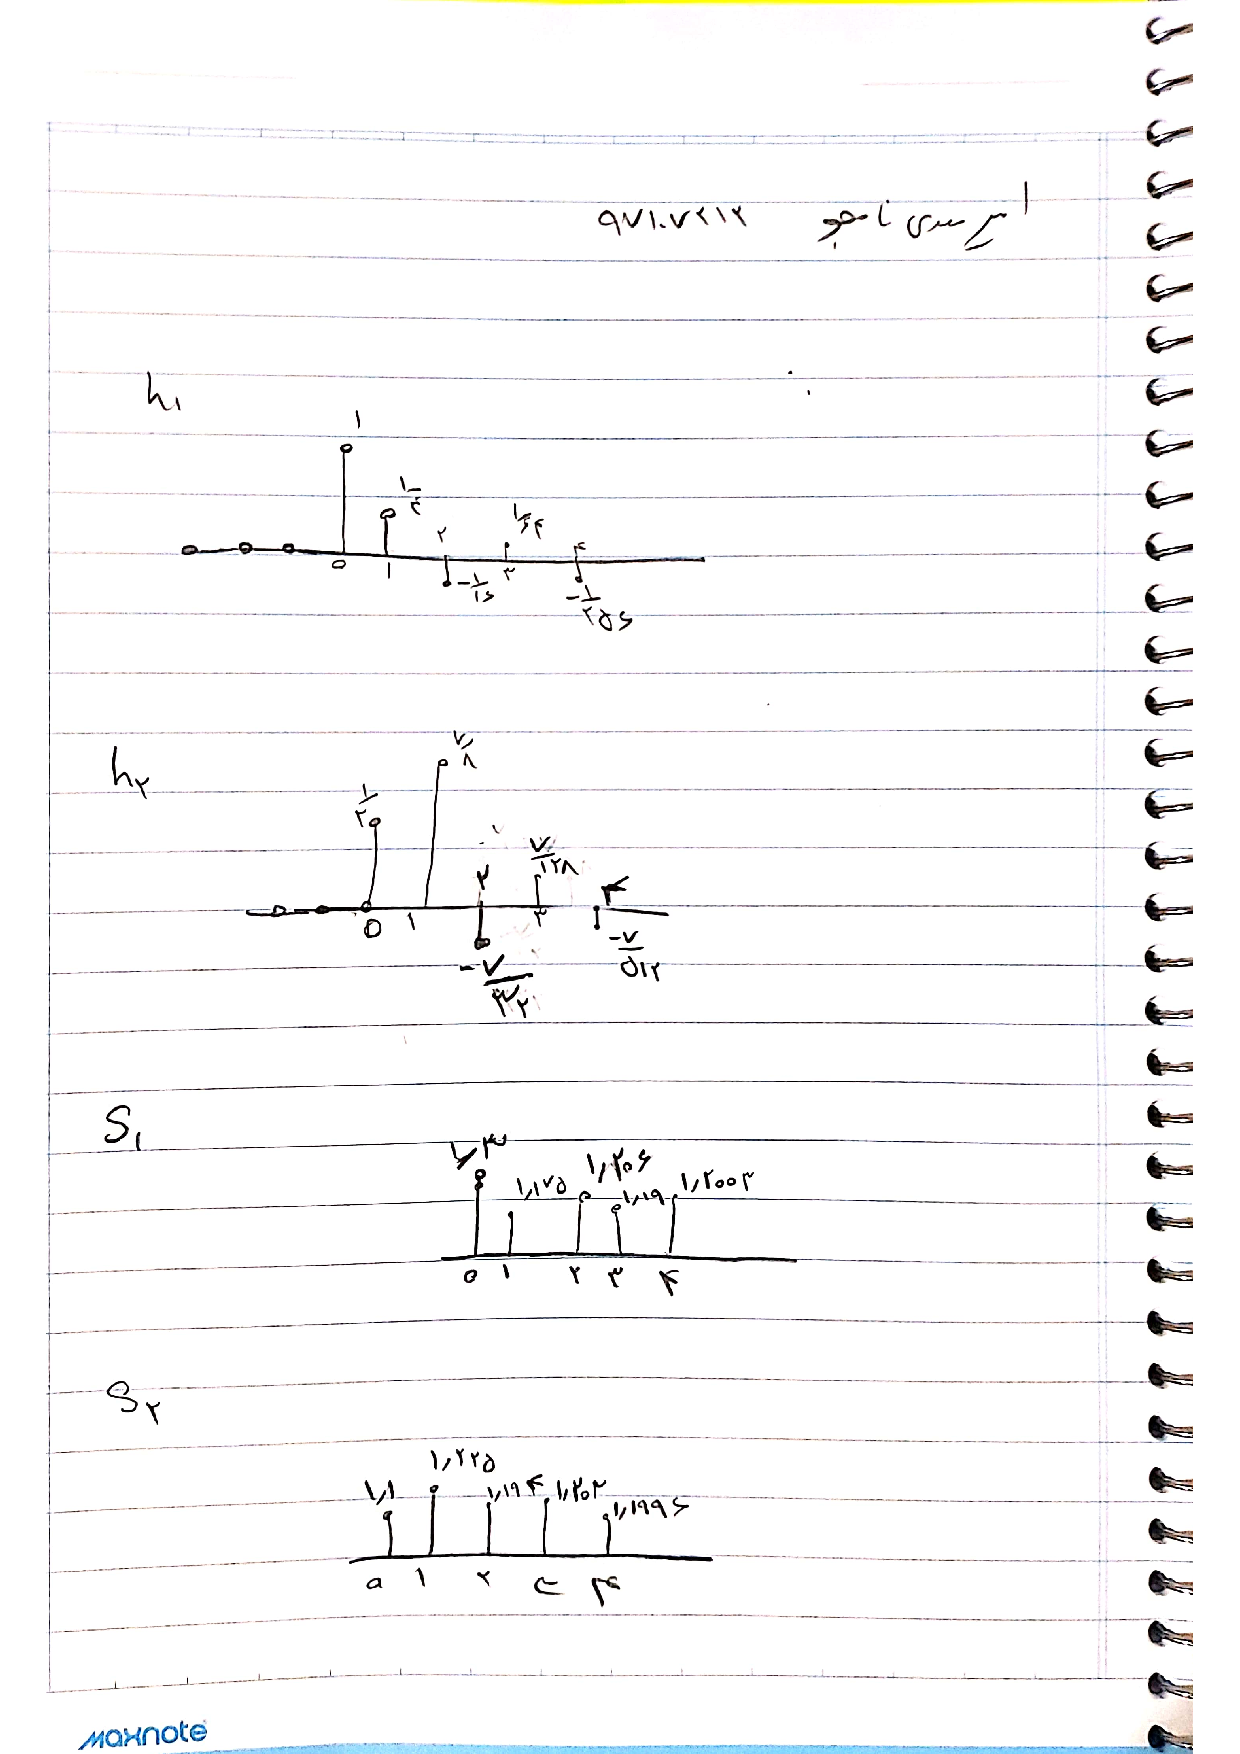
\includegraphics[width = 1.0\textwidth]{images/1.pdf}
\end{enumerate}

\newpage

\section{سوال دوم}

\begin{enumerate}
	\item 
	می‌توانیم فیلتر بالاگذر را به صورت زیر بنویسیم:
	
	$$H(j\omega) = 1 - H_0 (j \omega)$$
	که
	$H_0$
	مربوط به فیلتر پایین گذر است. با توجه به این که طبق کتاب فرمول مربوط به فیلتر پایین گذر را می‌دانیم داریم:
	
	$$h[n] = \delta(t) - h_0 (t) = \delta(t) - \frac{\sin \omega_c t}{\pi t}$$
	
	\item
	برای فشردگی نمودار کافیست به رفتار
	$$ \frac{\sin \omega_c t}{\pi t}$$
	نگاه کنیم. دو شکل زیر اولی برای $\omega_c = 4.6$ و دومی برای
	$\omega_c = 3.41$
	هستند. اولین نقاط برخورد نمودار با محور $t$ برابر
	$\pm \frac{\pi}{\omega_c} $
	هستند. با توجه به این موضوع با افزایش
	$\omega_c$
	متمرکزتر می‌شود.
	
	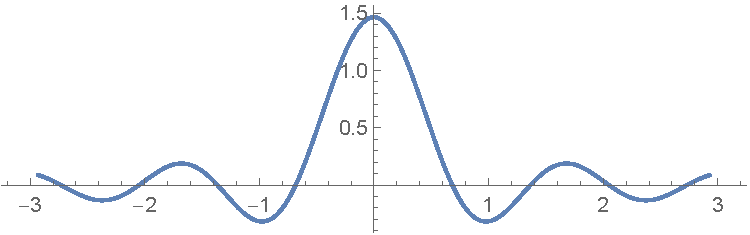
\includegraphics[width = 1.0\textwidth]{images/2.pdf}
	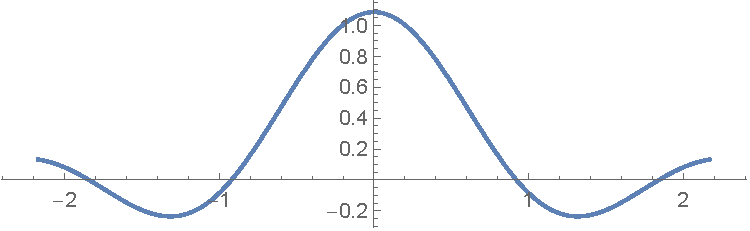
\includegraphics[width = 1.0\textwidth]{images/3.pdf}
	
	\item
	
	$$s(t) = h(t) \star u(t) = [\delta(t) - h_0 (t)] \star u(t) = u(t) - s_0(t)$$
	
	که 
	$s_0(t)$
	به شکل کامل در شکل $6.14$ کتاب رسم شده است.
	
	$$s(0+) = u(0+) -s_0(0+) = 1 - 0.5 = 0.5$$
	
	$$s(\infty) = u(\infty) - s_0(\infty) = 1-1 =0$$
	
	مقدار
	$s_0(0+),s_0(\infty)$
	از شکل کتاب استخراج شده‌اند.
	
	شکل کتاب در تصویر زیر هم قرار گرفته است:
	
	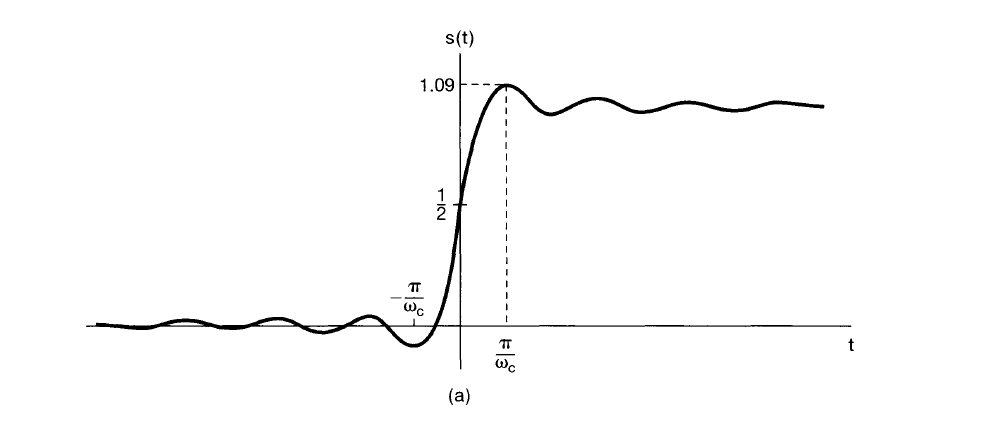
\includegraphics[width = 1.0\textwidth]{images/4.png}
	

	

\end{enumerate}

\newpage
\section{سوال سوم}
\begin{enumerate}
	\item 
	به نظر می‌رسد جزئیات رسم این سوال مربوط به فصل ۱۱ باشد. به هر حال با مطالعه
	
	  \href{https://ocw.mit.edu/courses/mechanical-engineering/2-004-dynamics-and-control-ii-spring-2008/}{ جزوه دینامیک و کنترل 2 دانشگاه \lr{MIT}}
	 ، به جواب زیر برای این سوال می‌رسیم:
	$$
	\frac{s-2}{(s+3)\left(s^{2}+2 s+17\right)}
	$$
	
	$$P_1 = -3$$
	$$P_{2,3} = -1 \pm 4 j$$
	$$z_1 = 2$$
	
	مقدار مماس عمودی به صورت زیر است:
	
	$$\alpha = \frac{\sum Pole - \sum Zero}{Num~ Pole - Num ~Zero} = \frac{(-3 - 1 -1) - (2)}{3 -1} = -3.5$$
	
	زاویه مماس به صورت زیر است:
	$$\angle \alpha = \frac{(2m+1) \pi}{Num~ Pole - Num ~ Zero}; m=0,\pm 1 , \pm 2,...$$
	$$\angle \alpha = \frac{(2m+1) \pi}{2} = \pm \frac{\pi}{2} $$
	
	
	شکل در صفحه بعد:
	
		\includegraphics[page = 2 , width=1.0\textwidth]{images/5.pdf}
	
	\item
	
	مخرج کسر  \lr{Closed Loop} تابع انتقال (معادله مشخصه) به صورت زیر است:
	
	$$1 + K H(s) = 0$$
	$$1 + K \frac{s-2}{(s+3)\left(s^{2}+2 s+17\right)} = 0$$
	$$(s+3)\left(s^{2}+2 s+17\right) + K(s-2) = 0$$
	$$
	s^{3}+5 s^{2}+(23+K) s+(51-2 K)=0
	$$
	
	برای معادله
	$$s^3 + a_2 s^2 + a_1 s + a_0 =0$$
	
	شرط پایداری روث-هورویتز به صورت:
	$$a_0 , a_1 , a_2 , a_2 a_1 - a_0 > 0$$
	است.
	
	$$a_0 = 51-2K > 0 \rightarrow K<25.5$$
	$$a_1 = 23 + K > 0 \rightarrow K>-23$$
	$$a_1 a_2 - a_0 = 7K + 64 >0 \rightarrow K>\frac{-64}{7}$$
	از صورت سوال هم داشتیم که $K>0$ پس در کل داریم:
	$$0<K<25.5$$ 
	
	
	\item
	$$H(s) = 
	\frac{2}{51}\left(\frac{s}{2}-1\right)^{1}\left(\frac{s}{3}+1\right)^{-1}\left[\left(\frac{s}{\sqrt{17}}\right)^{2}+\frac{2}{17} s+1\right]^{-1}
	$$
	
	$$Gain = \frac{2}{51} \approx -28 dB$$
	
	
	در بازه $\omega =0$ تا $\omega = 2$ زاویه $\pi$ است و مقدار ثابت.
	
	برای بازه $2$ تا $3$ ریشه داریم که شیب $20dB/dec$ و زاویه $\pi/2$ دارد.
	
	برای بازه $3$ تا $\sqrt{17}$ قطب داریم که شیب را $20dB/dec$ پایین آورده و $0$ می کند و زاویه هم $0$ رادیان.
	
	برای بازه $\sqrt{17}$ تا بی نهایت، قطب Underdamp شده مختلط داریم که $40dB/dec$ شیب را پایین آورده و زاویه $-\pi$ دارد.
	
	شکل اغراق شده رسم شده است تا تغییرات مشخص باشد. سعی شده شکل ها طوری رسم شود که تقریبا نقطه گذار $\sqrt{2}/2$ برای اندازه و نقطه وسط برای زاویه بر اعداد ریشه‌ها و قطب ها که در بالا آورده شده است، منطبق بشود. قطعا ولی به دلیل رسم شدن با دست شکل کاملا دقیق نیست.
	
	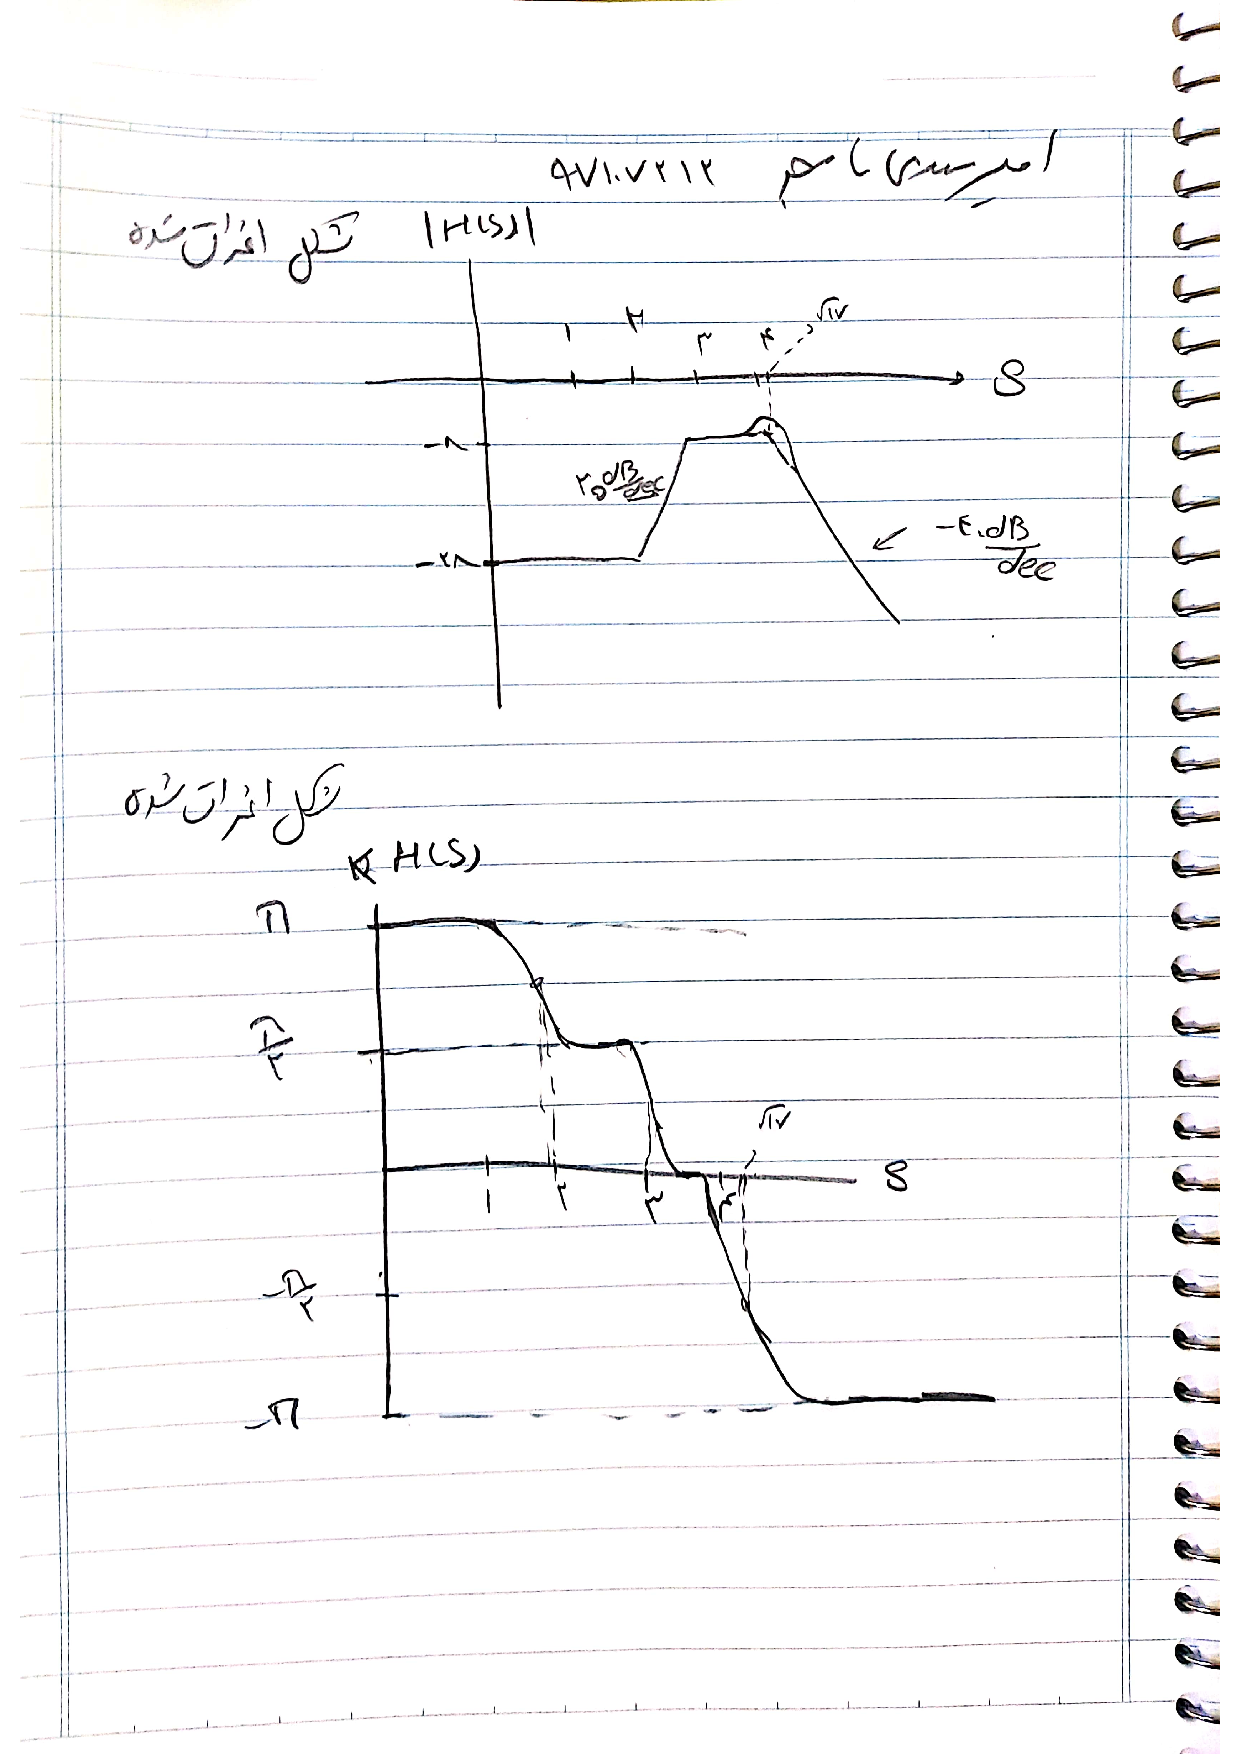
\includegraphics[page = 1 , width=1.0\textwidth]{images/5.pdf}
\end{enumerate}	
	
\end{document}



